\chapter{Proposal}
\label{Ch4}
\bigskip

Using the concepts of Block-Chain we propose our algoorithms for Image Integrity Analysis D-APP system.

We are trying to build a web-based social media application like WhatsApp and that will be connected with the online server running blockchain in it. The process of verification of the media (text, image or video) for checking fakeness or scam in a nutshell will be as follows,

As mentioned earlier, the main jobs of our project to build a small social media platform that will store images, show them in news feed and not only that, someone can bring an image and perform search operation in the system to check if we know about the image or not, i.e. if the image is valid or not.

The system we are proposing is a hybrid of previous strict systems in terms of Permission (Permissioned/Non-permisionalized) and Centralization (Centralized/Decentralized) along with some extra mechanisms. And also we preserve the scalability of the implementation that it is not necessary to have a dedicated huge computation power for all.

\section{Workflow}
The following is the control flow of the overall processes,
\begin{enumerate}
\item An user will have to log into the system first to be a part of the system;
\item There are two types of users, some are normal users and rest are miners who have some extra powers as well as responsibilities.
\item Normal users are those who will come to share their images by upload or taken from their camera interface and also search images for checking. In their home page they can scroll and click an image for viewing, search signatures, download images to own devices.
\item The miners are the creators of the blocks i.e. they will have computation power to generate the blocks, store the blocks in their own computers and broadcast them in the miners network, gossip among each others. They verify transactions before putting into a block.
\end{enumerate}

\section{System Design}
In one side of the system, the normal user can request the system either to store an image or to verify. On storing request the server will help the client's device to resize the image in a particular dimention (image preprocessing) and generate the correct request format in terms of transaction (Tx). Then the server will create a copy of it making a symmetric key encryption over assymetric key encryption of the user and store in own file system database in unverified or new transaction file.

On a certain time interval (not so long, not so small, bitcoin takes 10 minutes, we will take it 5 minutes) the miners will be verifying these pool of unverified transactions and adding them in new blocks in parallel through consensus mechanism. Our consensus mechanism works as follows,

\begin{figure}
\begin{center}
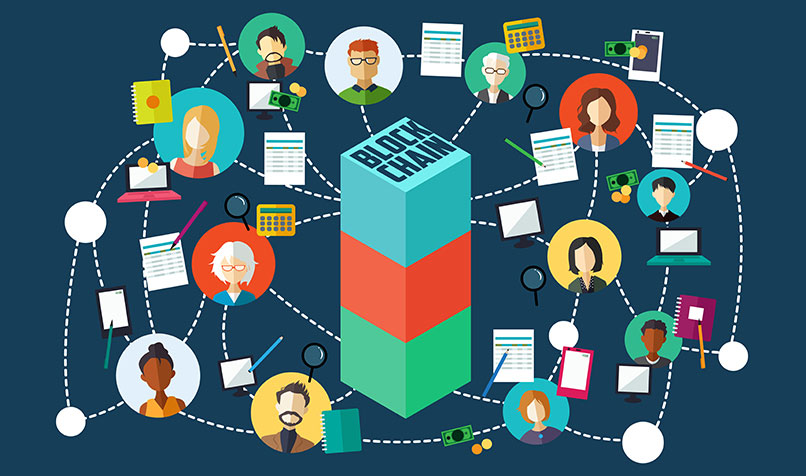
\includegraphics[width=0.75\textwidth]{./img_src/blockchain_network.jpg}
\end{center}
\caption{Consensus mechanism}
\end{figure}

\subsection{Consensus mechanism}
\begin{enumerate}
\item At a time interval the server will broadcast the transactions or the miners will get them on request from the server database through XML-HTTP or SFTP protocol.
\item The miners either individually or by gossiping will verify the transaction data. Verifying by own will create the uniqueness, by gossiping maintains the correctness that prevent the fault from any side (server, other miners, itself).
\item After they delete the invalid transaction set they will start creating new block out of it.
\item After a node discovers or completes creating a new block, it broadcasts to the miner network and waits for confirmation and others blocks. After a node gets a new block, it holds it's own computation and validate the new block. If the new block is valid and the node have all previous blocks that should be linked in the chain by previous hash the node keeps it into own temporary space, and wait for others for confirmation, and if not valid then resume own computation. After all blocks say we have a valid block (either own or someone else's) to each other, they compare with what other nodes are having. The winner is one of the blocks which is having most of the criterias below,
\begin{enumerate}
\item Biggest in size $\implies$ It is having maximum number of transactions
\item Bigger nonce $\implies$ Most computation power is spent for it.
\item Lowest rewarded miner $\implies$ To remove partiality and create balance and good understanding between miners.
\end{enumerate}
After 5 minutes the server requests the miners to get the decided block to be added in the chain. Server validates the block and adds it in the chain and remove the transactions that are either added or marked as invalid from the transaction pool.

\begin{figure}
\begin{center}
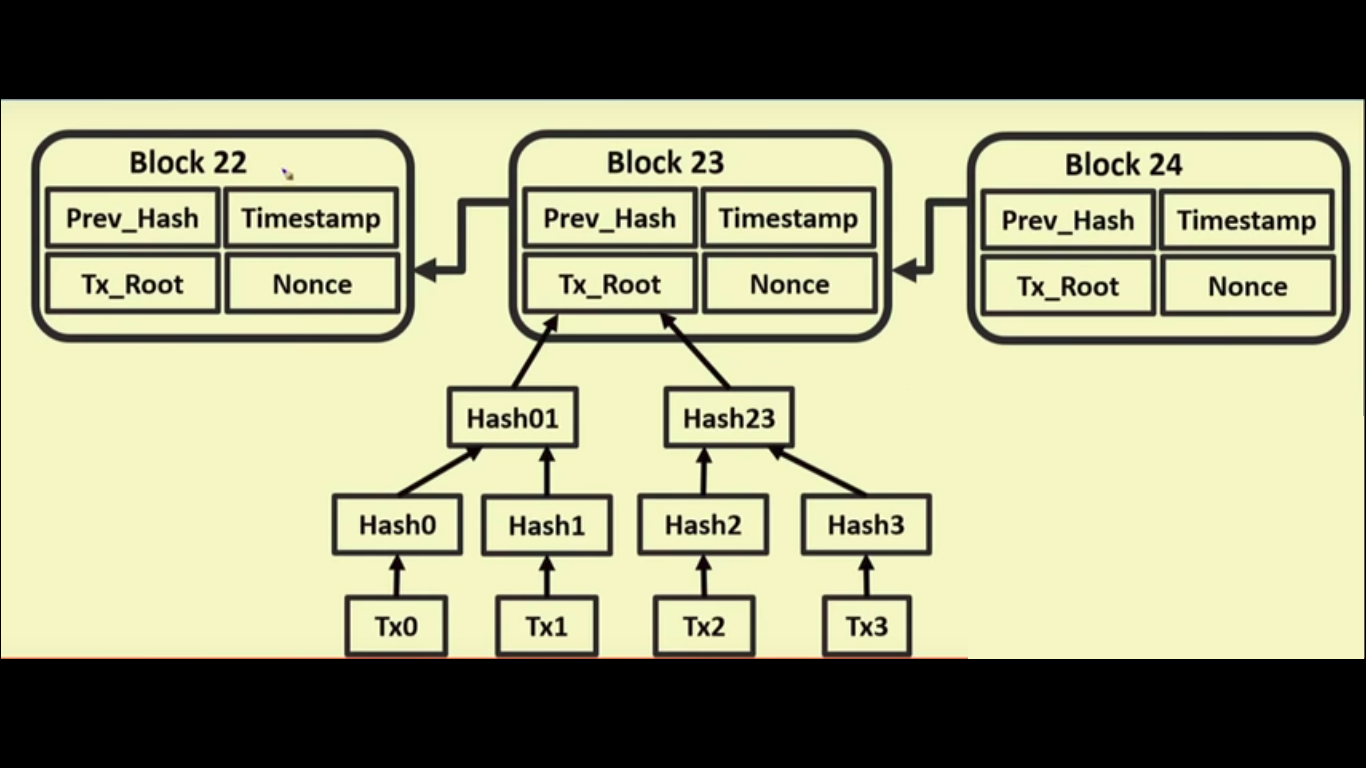
\includegraphics[width=0.75\textwidth]{./img_src/block_chain.png}
\end{center}
\caption{Block Creation}
\end{figure}

\item On request of an image verification, first the image metadata is being checked (1st phase). If the metadata contains the our system generated signature, it will decrypt it and check in that particular block or the range of the blocks for the transaction that contains the image as well as the user's profile for it. Becacuse while creating downloadable file the system encrypts and adds the metadata in the image file. If found, it generates the confirmation message and the links regarding it. And if not then the system requests for time and search the entire blockchain database for hashes (2nd phase). If found it does the same. And still if it not found, it runs a deep CNN for searching for contexts or by object for maximum possible proof (3rd phase). The result it gives now is the final result.
\item The process continues again and again recursively.
\end{enumerate}
